\begin{table*}[h]
\centering
\caption{Accuracy of different speech recognition services and accents against the audio captcha services we evaluated.}
\begin{tabular}{lccccc}
\toprule
&\multicolumn{5}{c}{\textbf{Speech Recognition Service (Accent)}}\\
\cmidrule{2-6}
\textbf{Captcha Service}& \textbf{Wit}& \textbf{IBM (US)} & \textbf{ IBM (UK)} & \textbf{Google (US)} & \textbf{Google (UK)} \\
\hline
Recaptcha v2.0 & 67.1\% (671/1000) & 95.8\% (958/1000) & 67.2\% (672/1000) & \textbf{98.3\%} (983/1000) & 81.6\% (816/1000) \\
\rowcolor{Gray}
Recaptcha v2.1 &  &  &  &  & \\
Apple  & 0\% (0/365)  & 2.3\% (6/260) & 6.8\% (17/251) & 35.8\% (126/352) & \textbf{52.8\%} (143/271) \\
\rowcolor{Gray}
BotDetect  & 1.23\% (11/894)  & 1.38\% (19/138) & 6.67\% (12/180) & \textbf{9.5\%} (102/1067)  & 6.65\% (79/1187) \\
Captchas.net  & 0\% (0/1008) & 1.1\% (9/778)  & 0.3\% (3/1010)  & 2.7\% (16/593) & \textbf{22.3\%} (230/1030) \\
\rowcolor{Gray}
Microsoft Live & &  &  & & \\
Securimage  & 0\% (0/1000)  & 0\% (0/1000) & 0\% (0/1000) & 0.1\% (0/1000) & \textbf{3\%} (30/1000) \\
\rowcolor{Gray}
Telerik  & 21.2\% (142/668)  & \textbf{97\%} (452/466) & 12.9\% (47/364) & 74.2\% (150/202) & 49.3\% (112/217) \\
\bottomrule
\end{tabular}
\label{tab:combinations}
\end{table*}

\section{Experimental Evaluation}
\label{sec:evaluation}

In this section we present the results from our extensive experiments again 
the audio captcha services presented in Section~\ref{sec:services}.

\textbf{Attack accuracy.} Table~\ref{tab:combinations} presents the accuracy obtained by each speech recognition service 
against the audio captcha services. In cases where the speech recognition service has the option to select an accent,
we experiment with both American and British English. Surprisingly, we find that for every single captcha scheme, at least
one of the speech recognition services is able to solve more challenges than the 1\% threshold, thus, \emph{practically 
rendering all captcha schemes broken.} Nonetheless, there is significant variance, not only across captcha schemes, but
the accuracy obtained by each speech recognition engine for a specific captcha service. 

The most alarming finding is 
that \system achieved the highest accuracy against \re v2.0, the most widely deployed captcha service. When compared 
to the 70.78\% attack accuracy reported for the image \re~\cite{sivakorn:eurosp16}, it becomes apparent that audio challenges
weaken the overall security offered by \re, as fraudsters can target audio captchas for deploying highly successful
attacks. The Apple and Microsoft Live captchas that protect their account creation process, are also highly susceptible to 
automated attacks, as our approach correctly solves up to \note{52.8\% and X\%} respectively.

Despite the presence of noise impacting the accuracy of the transcription process for all the respective captcha schemes
(see Table~\ref{tab:services}), none of the services is completely impervious to our attacks. Nonetheless, we
found that the audio captchas from Securimage are the most robust due to the presence of background semantic noise,
as \system was only able to solve 3\% of the challenges when using Google's Speech API and the British English accent
configuration. Another interesting observation was that no single speech recognition system or configuration
was consistently more accurate across all captchas; however, Google's speech recognition achieved the best
results for \note{X} out of the \note{Y} captcha schemes. While attackers could increase the attacks' accuracy
by first pre-processing the audio challenges so as to reduce the noise, the motivation behind our study is to 
demonstrate how attackers can employ off-the-shelf systems for breaking existing captcha systems.
Based on these results, we find that \system would be an effective replacement to the human solvers employed by
captcha solving services, as humans are often troubled by audio captchas~\cite{captchas-are-hard}.


\begin{table}[t]
\centering
\caption{Average solution time for each recognition service and accent against the audio captcha services we evaluated.}
\begin{tabular}{lccccc}
\toprule
&\multicolumn{5}{c}{\textbf{Speech Recognition Service}}\\
\cmidrule{2-6}
& & \textbf{(US)} & \textbf{(UK)} & \textbf{(US)} & \textbf{(UK)} \\
\textbf{Captcha}&  \textbf{Wit} & \textbf{IBM} & \textbf{IBM} & \textbf{Google} & \textbf{Google} \\
\hline
Recaptcha v2.0 & 13.85s & 10.56s  & 12.25s & \textbf{18.46s} & 20.41s \\
\rowcolor{Gray}
Recaptcha v2.1 &  &  &  & & \\
Apple  & 36.4s & 33.4s  & 34.7s & 15.5s & \textbf{13.9s} \\
\rowcolor{Gray}
BotDetect  & 5.53s  & 4.21s & 5.72s & \textbf{3.40s} & 3.05s \\
Captchas.net  & 19.92s  & 14.62s  & 15.65s  & 7.56s & \textbf{7.79s} \\
\rowcolor{Gray}
Microsoft Live & &  &  & & \\
Securimage  & 34.31s & 23.60s & 25.10s  & 27.29s & \textbf{35.28s} \\
\rowcolor{Gray}
Telerik  & 7.53s & \textbf{5.56s} & 6.65s & 3.86s & 3.83s \\
\bottomrule
\end{tabular}
\label{tab:solution_time}
\end{table}

\textbf{Solution time.} In Table~\ref{tab:solution_time} we include the average time required by each speech recognition 
service for returning a transcription of the audio captcha. The bold values denote the combination that achieved the highest 
accuracy for that captcha scheme. \note{Talk about results.}

\note{How many mistakes allowed for a correct answer?}

\textbf{Rate limits and economic analysis.} Our study's goal is to explore the feasibility of low-cost attacks 
against popular captcha services; thus, the scale of such an attack is naturally constrained by the rate
limiting enforced by the speech recognition APIs. While an attacker could build an offline solver
using a deep learning framework like TensorFlow~\cite{abadi2016tensorflow}\footnote{Researchers have already
released prototypes that build on Tenserflow: {https://github.com/mozilla/DeepSpeech}.} to overcome this constraint,
our threat model explicitly includes non-sophisticated attackers that do not develop or train their own 
classifiers. As such, the rate limits of each speech recognition service become relevant as they could
constrain our attacks.

\begin{table}[t]
\centering
\caption{Attacker's estimated daily profit for each captcha service, when using one Google Speech API account
(with the most accurate accent configuration for that captcha scheme).}
\begin{tabular}{lccc}
\toprule
& \textbf{Captcha} & \textbf{Estimated} & \textbf{Daily} \\
\textbf{Captcha}&  \textbf{Duration} & \textbf{Solutions} & \textbf{Profit} \\
\hline
Recaptcha v2.0 & 7 sec & 242,413 & \$485.3 \\
\rowcolor{Gray}
Recaptcha v2.1 & 15 sec & & \\
Apple  & 14 sec & 65,170 & \$130.3 \\
\rowcolor{Gray}
BotDetect  & 6 sec & 28,215 & \$54.7 \\
Captchas.net & 14 sec & 27,524 & \$55 \\
\rowcolor{Gray}
Microsoft Live & & & \\
Securimage & 10 sec & 5,184 & \$10.3 \\
\rowcolor{Gray}
Telerik & 7 sec & 188,892 & \$366.3 \\
\bottomrule
\end{tabular}
\label{tab:money}
\end{table}

Surprisingly, these services have very lax limits that would enable fraudsters to misuse
them for maintaining large scale audio captcha solving campaigns. For instance, Google's Speech API allows up
to 250,000 requests per day, where multiple audio files can be submitted per request, allowing for a maximum of
480 hours of audio processing\footnote{https://cloud.google.com/speech/limits}. 
In Table~\ref{tab:money} we provide a rough estimation of the profit that an attacker could yield against 
each captcha service per day using a single Google API account. We assume a lower end market price of \$2 
per 1,000 solved captchas, and calculate the number of solved captchas based on the length of audio challenges 
and the highest accuracy achieved by a Google Speech solver (see Table~\ref{tab:combinations}) for each service.
\note{Most noteworthy results.} It is important to note, however, that these calculations assume that the attacker 
is not constrained by other forms of rate limiting (e.g., IP-based limits). Given the workarounds employed
by existing captcha solving services (e.g., proxies, botnets, etc), in practice these limitations will not 
pose insurmountable obstacles.

On the other hand, IBM Watson allows 1 free month per account\footnote{https://www.ibm.com/watson/services/natural-language-classifier/}.
Finally, Wit does not have an explicit rate limit. However, it is open to commercial
apps and requests notification for rates approaching one request per second. As all three services
only require an email address for creating an account, attackers could trivially register 
new email addresses periodically for increasing their overall allowed throughput.

%In comparison Clarifai,
%the most accurate image annotation service used against \re~\cite{sivakorn:eurosp16}, only allows 5,000
%free operations per month\footnote{https://developer.clarifai.com/pricing/}.


\textbf{Solution flexibility.} \note{How many wrong digits allowed per service?}

\begin{figure*}[t]
\begin{subfigure}{0.75\textwidth}
    \centering
    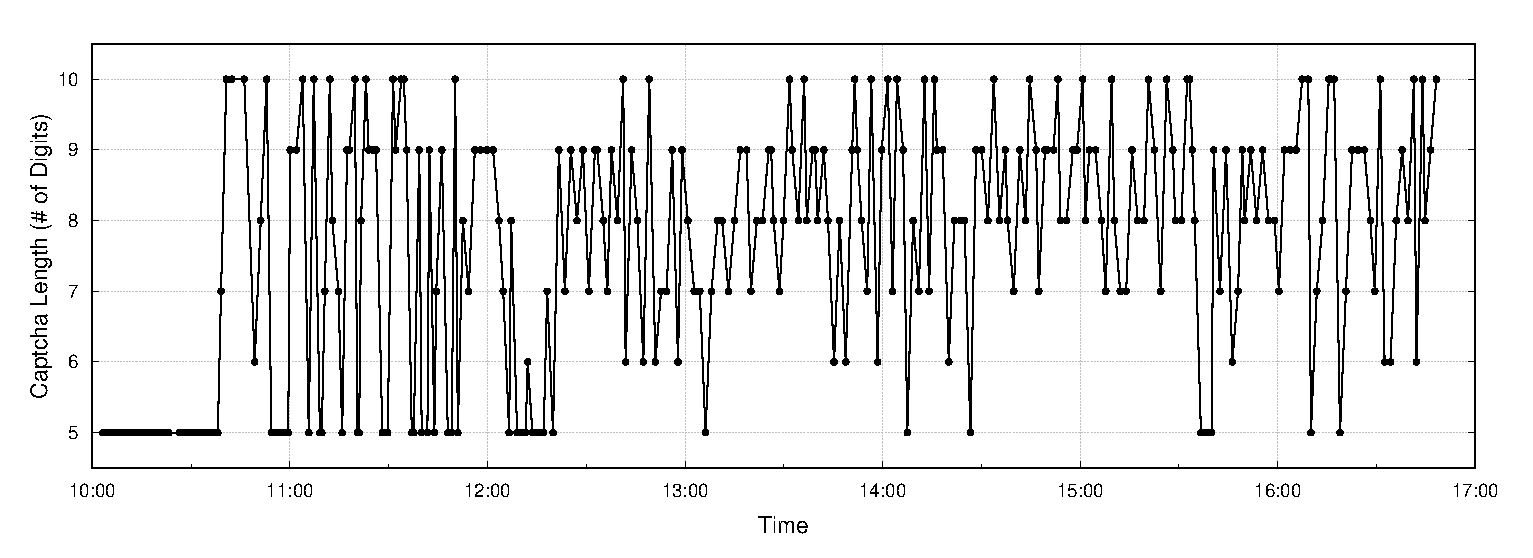
\includegraphics[width=1\textwidth]{figures/captcha_length.eps}
    \label{fig:length_time}
\end{subfigure} %\hspace{0.03\textwidth}
\begin{subfigure}{0.2\textwidth}
    \centering
    %\caption{Average solution time for each recognition service and accent against the audio captcha services we evaluated.}
    \label{tab:length}
    \begin{tabular}{lc}
    \toprule
    \textbf{Digits} & \textbf{\# of Captchas} \\
    \hline
    5 & 95 (31.3\%) \\
    \rowcolor{Gray} 
    6 & 14 (4.6\%) \\
    7 & 34 (11.2\%) \\
    \rowcolor{Gray} 
    8 & 51 (16.8\%) \\
    9 & 68 (22.4\%) \\
    \rowcolor{Gray} 
    10 & 41 (13.5\%)\\
    \bottomrule
    \end{tabular}
\end{subfigure}
\caption{Variation of audio captcha length in \re v2.0 over time.}
\label{fig:length}
\end{figure*}

\textbf{\re.} While our study aims to evaluate the robustness of many popular audio captchas, 
Google's \re is the most prevalent captcha service, so we offer some interesting details 
and findings from our experiments.

\emph{Bypassing rate limits.} As aforementioned in Section~\ref{sec:recaptcha}, \re enforces 
rate limiting to prevent large scale attacks from a small number of machines. While in practice
captcha solving services employ proxies~\cite{captcha_proxies} and botnets (e.g., KoobFace~\cite{captcha_solvers}) 
to overcome such limits, we further explored this mechanism during our experiments. Initially,
we employed a straightforward approach of circulating through a list of valid User Agent strings,
so as to masquerade as numerous computers connecting from a single IP address (e.g., users behind a NAT).
However, in that case \re would enforce the same limit. Surprisingly, though, we found that if we 
supplied a bogus nonsensical User Agent we were able to completely bypass the rate limiting,
and only faced issues when issuing many concurrent solvers (which could appear as a potential DDoS attempt).
%solving  well over a thousand captchas per day from a single IP address. 
We surmise that a bug in the risk analysis
system does not enforce the check on the other aspects of the request (e.g., IP address, HTTP cookies) when
it encounters an ``invalid'' User Agent\footnote{This issue has now been fixed.}.
%This incident 
%further highlights how seemingly complex captcha services ]

\emph{Adaptive length}.
While by default the length of \re v2.0 was 5 digits, we found %that after multiple captcha solutions by our system,
that \re would adapt when facing a large amount of requests from our system and return captchas with more digits. 
In Figure~\ref{fig:length} we present a representative experiment that depicts the number of digits in the captchas
processed by our system over the course of 7 hours. The first 49 captchas all contained 5 digits, whereas the length
changed in a seemingly random fashion. As can be seen by the breakdown statistics in the figure, apart from the default
version with 5 digits, the most common variation we came across contained 9 digits.
%Overall, out of the 303 challenged processed in the experiment, 95 (31.3\%)
%had a length of 5, 14 (4.6\%) had 6 digits, 34 (11.2\%) had 7, 51 (16.8\%) had 8 digits, 68 (22.4\%) had 9, and 41 
%(13.5\%) had 10 digits.

\begin{figure*}[tp]
\begin{subfigure}{0.24\textwidth}
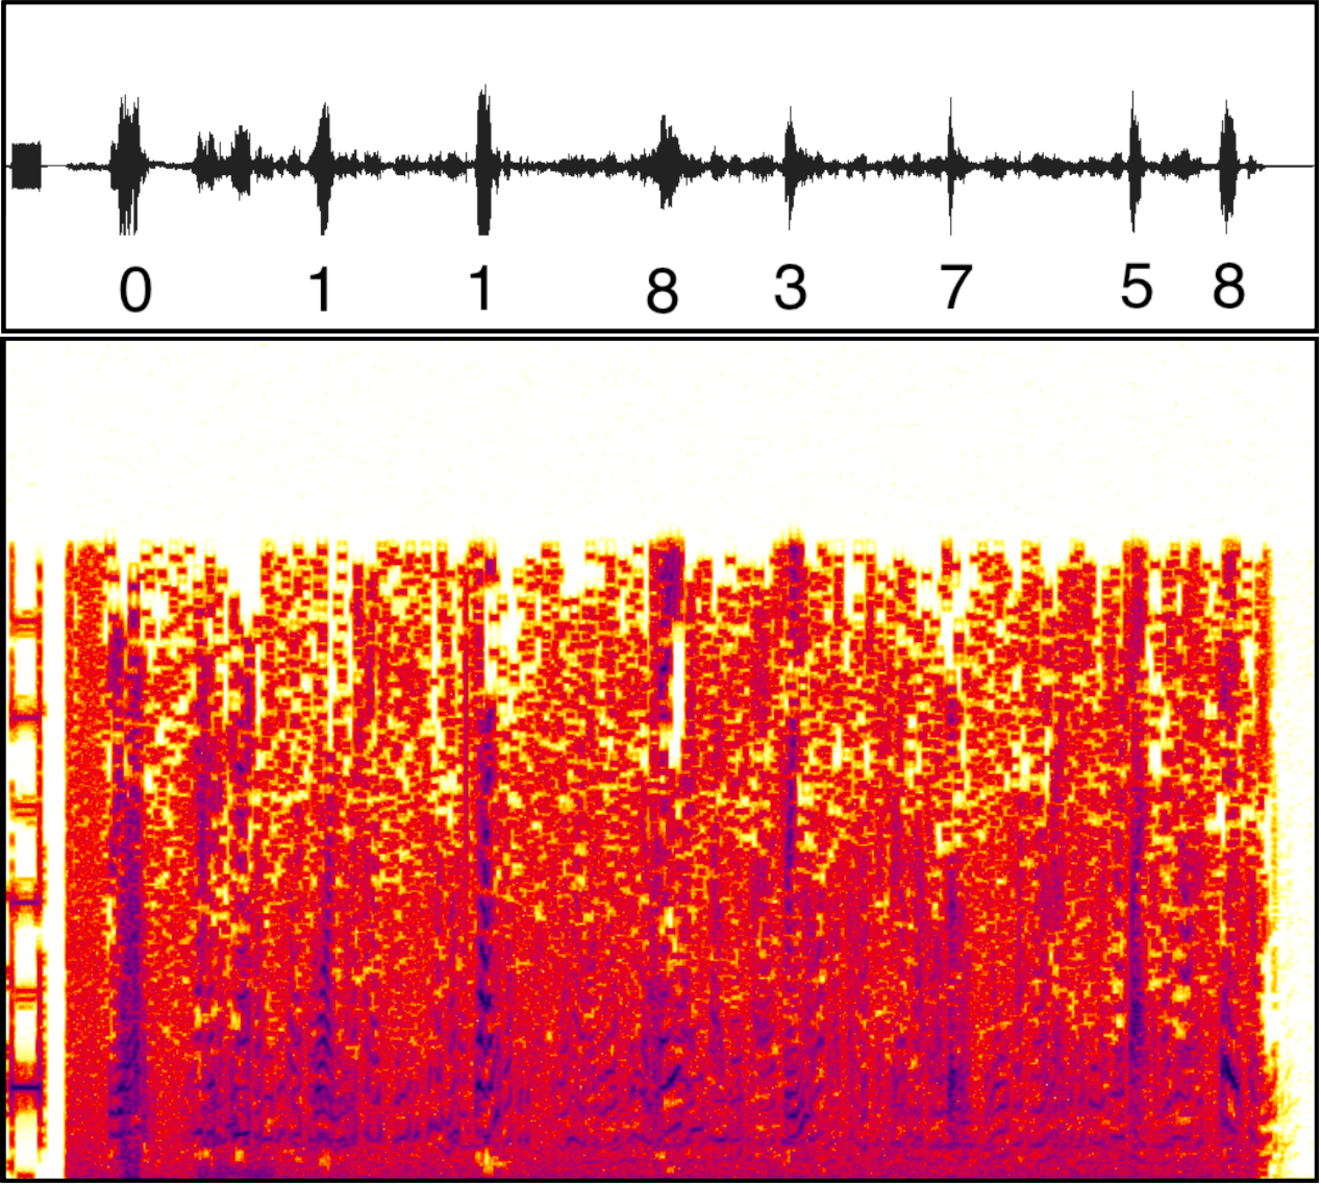
\includegraphics[width=\textwidth]{figures/recaptcha_evolution/2011.pdf}
\caption{\re cca. 2011}
\label{fig:apple}
\end{subfigure} \hspace{0.01\textwidth}
\begin{subfigure}{0.24\textwidth}
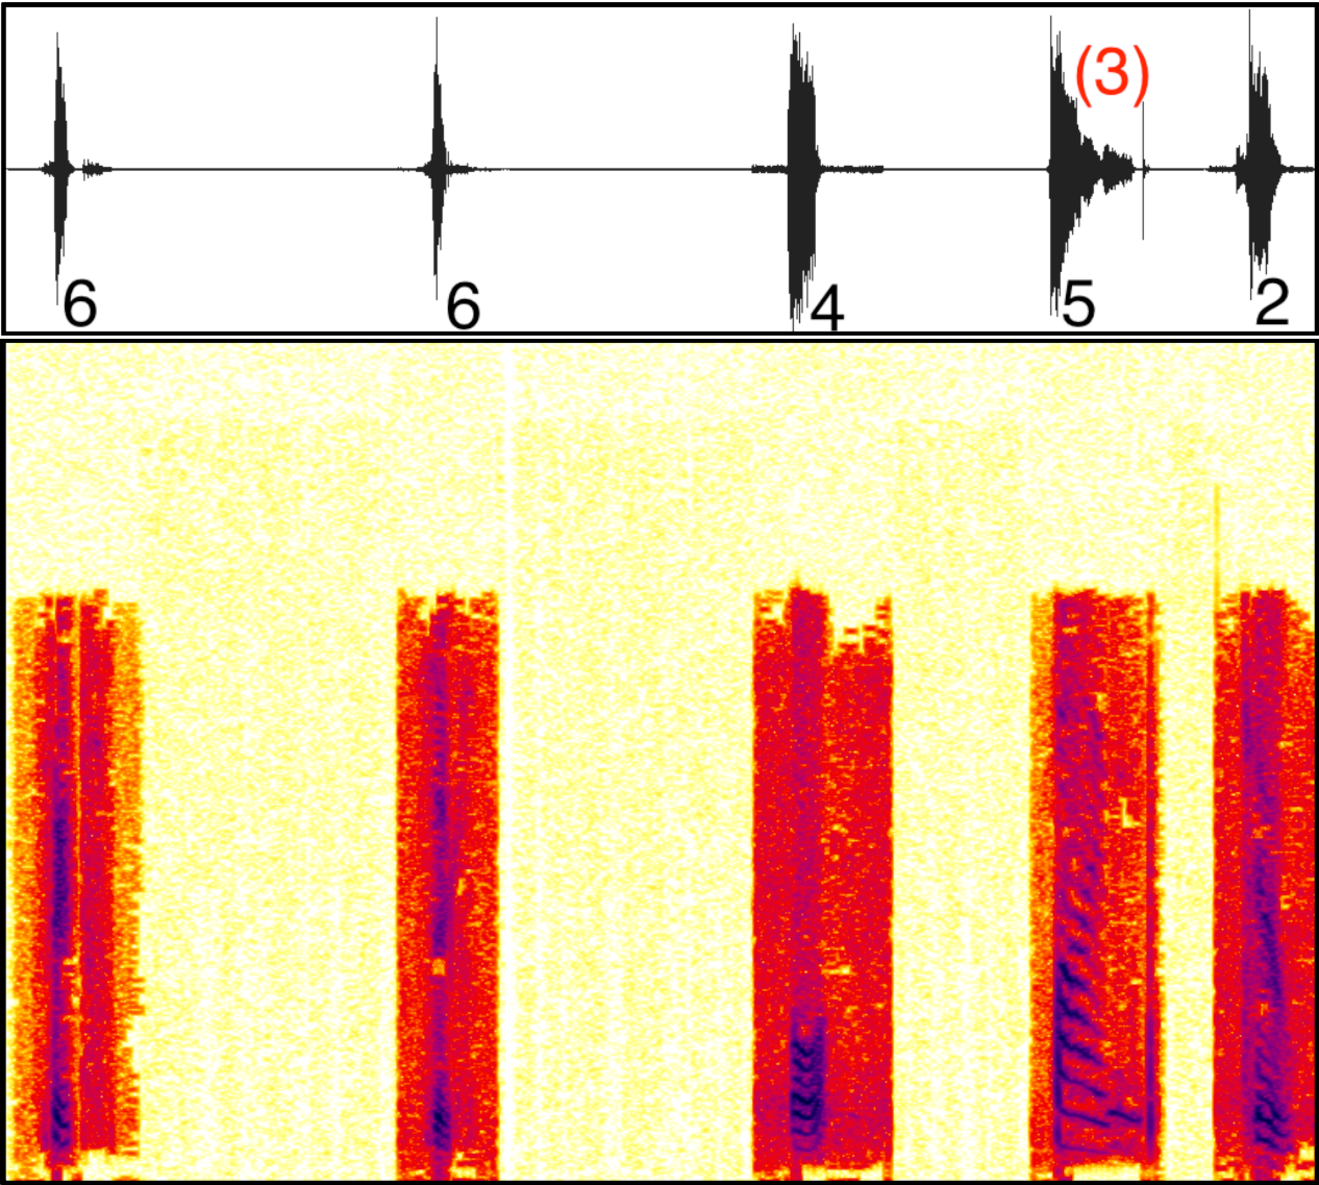
\includegraphics[width=\textwidth]{figures/recaptcha_evolution/2014b.pdf}
\caption{\re cca. 2014}
\label{fig:botdetect}
\end{subfigure}\hspace{0.01\textwidth}
\begin{subfigure}{0.24\textwidth}
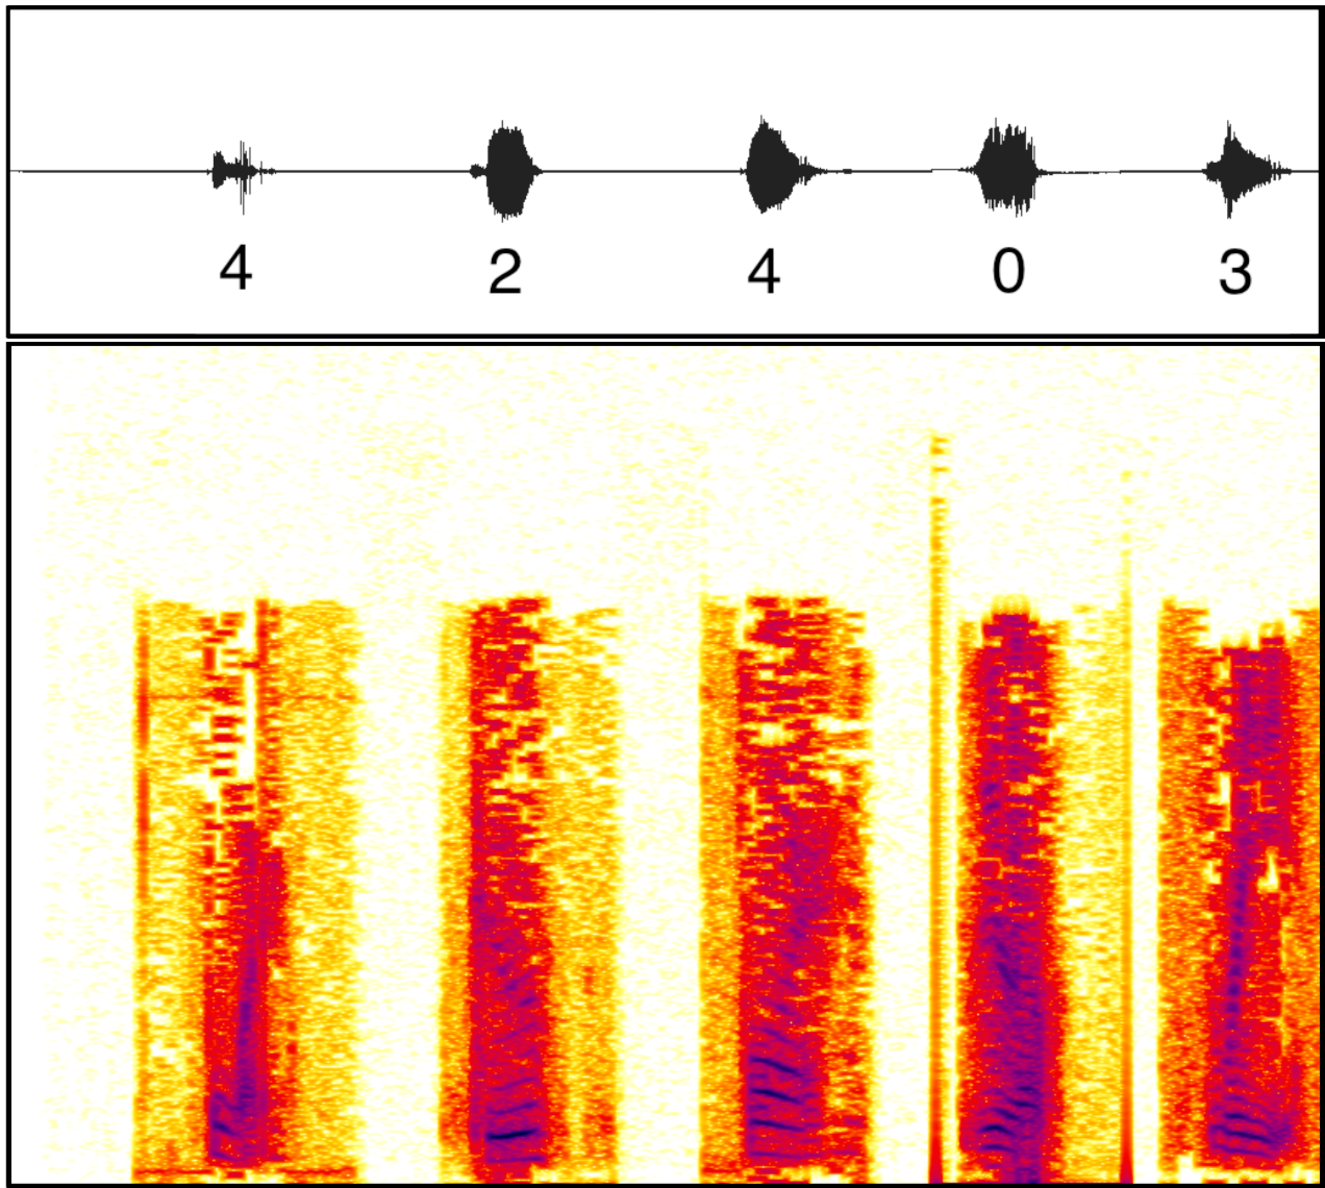
\includegraphics[width=\textwidth]{figures/recaptcha_evolution/2016.pdf}
\caption{\re cca. 2015-2016}
\label{fig:captchas}
\end{subfigure}
\begin{subfigure}{0.24\textwidth}
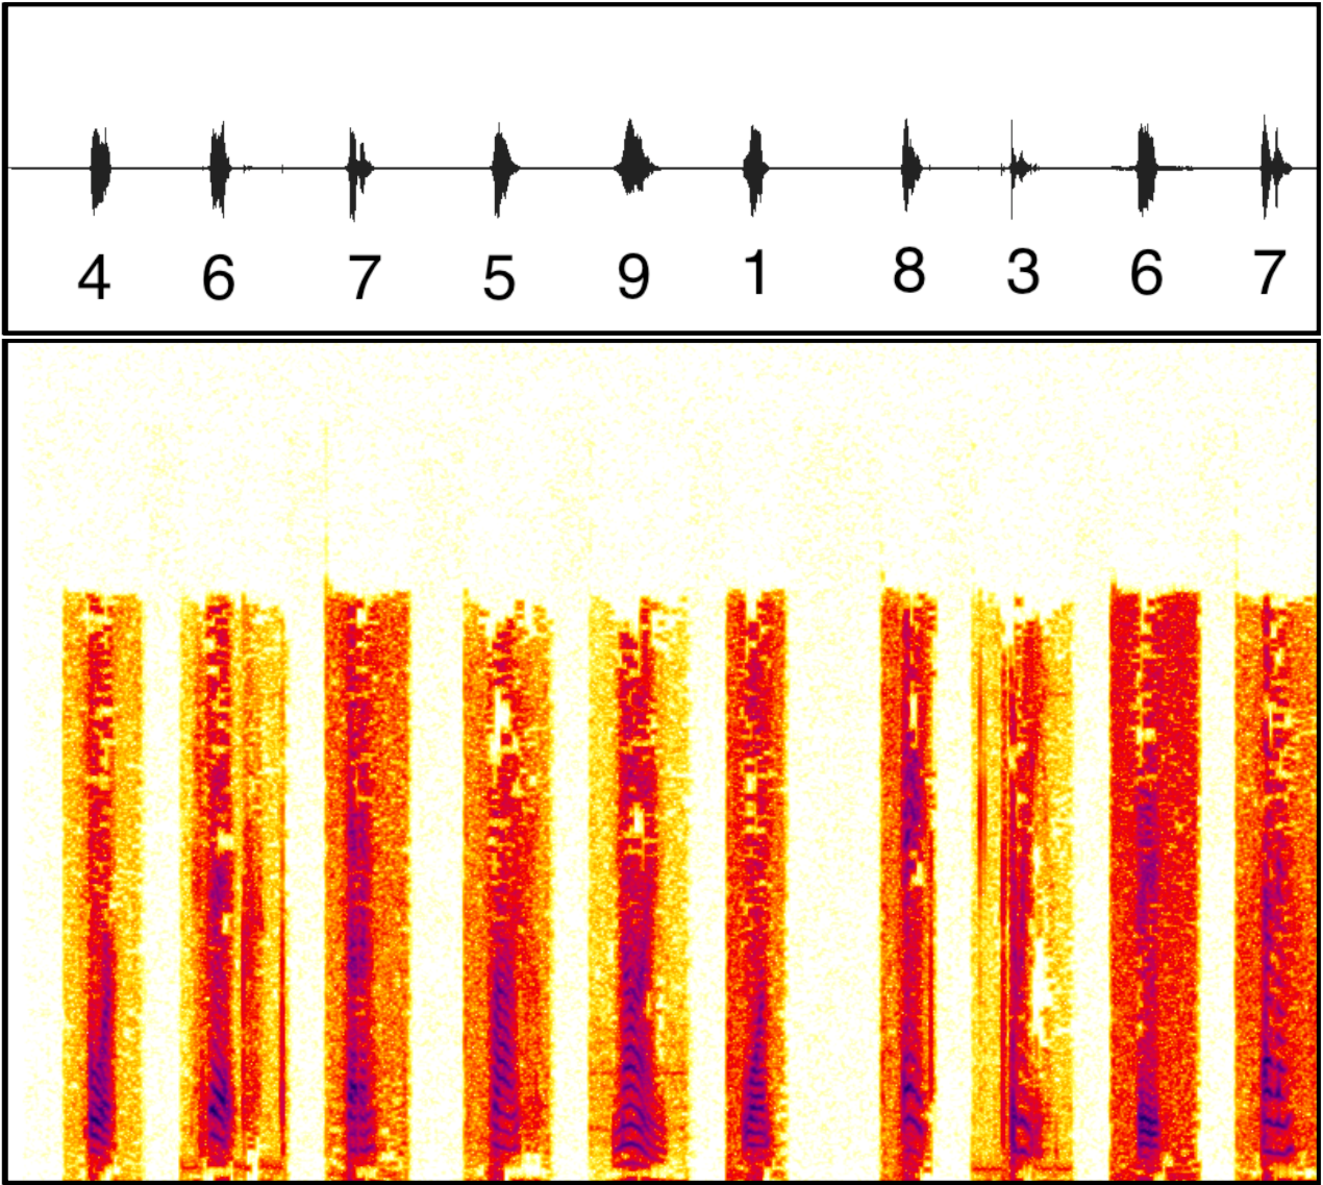
\includegraphics[width=\textwidth]{figures/recaptcha_evolution/2017.pdf}
\caption{\re after March 2017}
\label{fig:live}
\end{subfigure}
\caption{The evolution of \re audio challenges through time.}
\label{fig:evolution}
\end{figure*}


\emph{Evolution through time.} In their extensive user study on the usability of captchas, Burzstein et al.~\cite{captchas-are-hard}
found that users were able to solve only 47\% of \re's audio challenges (that number was calculated following an optimistic approach
and is an upper bound to the actual accuracy). Since then \re has modified their audio challenges. % to be more user friendly.
Here we further explore how audio \re has evolved through time. 

In Figure~\ref{fig:evolution} we visualize audio captcha samples
that capture \re's evolution through time. Indeed, the audio challenges from 2011 are the least ``user-friendly'' as they contain
a significant amount of background noise in the form of unintelligible discussions, reversed recordings of speech. While the version
from 2014 is considerably clearer and only five digits long, the audio quality of the spoken digits remains ``noisy'', while background recordings were
also sporadically interjected. In the sample plotted here, a background recording uttering ``three'' is almost overlapping with the
digit spoken as part of the challenge (shown in red). As part of their ``No Captcha Recaptcha'' system released in December 2014, the audio challenges were 
more simplified as they contained five digits with less noise in the recordings; however, certain recordings are processed and the sounds
are more drawn out. This could potentially be a countermeasure against automated attacks. 
Finally, in the current version which was released in March 2017,
the challenges once again contain 10 digits. 

While there might have been more intermediary changes apart from the ones presented here,
this samples show a clear evolution of audio \re challenges towards a more user-friendly scheme. The change in the latest version 
is most likely an attempt to mitigate automated attacks; however, this can only serve as a temporary measure as our experiments
demonstrate that speech recognition technology has reached a point where such challenges can be trivially bypassed. Thus, it remains 
to be seen whether \re adopts an approach similar to services like Securimage and BotDetect and reverts back to challenges with 
more noise and distortion to hinder automated attacks.
